\documentclass{fizykalab}

% Ustawienia do tabelki

\wydzial{WI}
\autorjeden{Dawid Komęza}
\autordwa{Magdalena Śmietana}
\rok{II}
\grupa{14}
\zespol{2}
\temat{}
\nrcwiczenia{}
\datawykonania{}
\dataoddaniajeden{}
\zwrotdopoprawy{}
\dataoddaniadwa{}
\datazaliczenia{}

\begin{document}

\maketitle
\section{Cel ćwiczenia}
Celem ćwiczenia jest poznanie podstawowych właściwości pola elektrostatycznego oraz zasad jego modelowania. Zadanie obejmuje doświadczalne wyznaczenie powierzchni ekwipotencjalnych i odpowiadających im wektorów natężenia pola elektrycznego dla różnych konfiguracji elektrod.
Dodatkowo, celem jest utrwalenie pojęć dotyczących pól wektorowych, praw Gaussa i Coulomba, rozkładu ładunku w przewodnikach, a także zależności między potencjałem a natężeniem pola elektrycznego.

\section{Wstęp teoretyczny}
Pole elektrostatyczne jest przykładem \textbf{pola źródłowego}, wytwarzanego przez nieruchome ładunki elektryczne. Do pól tego typu należą również pole grawitacyjne czy pole prędkości cieczy wypływającej ze źródła. Charakterystyczną cechą pól źródłowych jest to, że linie sił rozpoczynają się w źródłach (ładunkach dodatnich) i kończą w zlewach (ładunkach ujemnych).
Dla porównania, przykładem \textbf{pola wirowego} jest pole magnetyczne – jego linie są zawsze zamknięte i nie mają początku ani końca. Inne pola wirowe spotyka się np. w przepływach cieczy i gazów (wir, tornado).

\begin{figure}[h!]
\centering
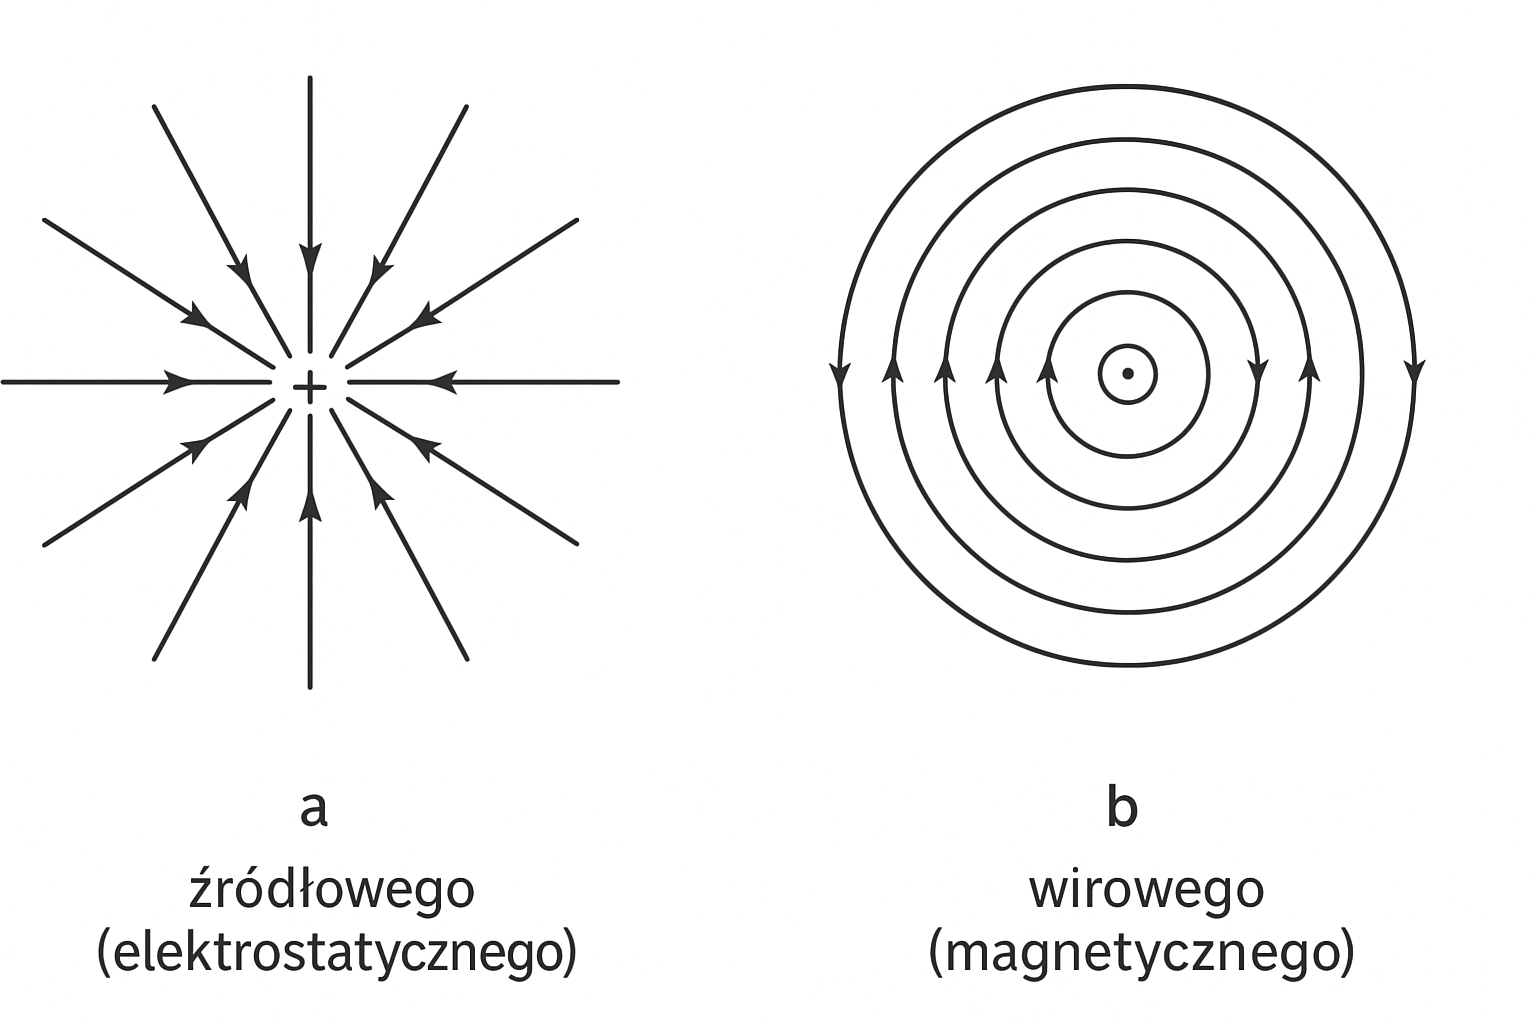
\includegraphics[width=0.8\linewidth]{rysunek1.png}
\caption{Przykładowe linie pola: a) źródłowego (elektrostatycznego), b) wirowego (magnetycznego)}
\end{figure}

\subsection*{Prawo Coulomba i prawo Gaussa}
Podstawowym prawem opisującym oddziaływanie ładunków punktowych jest \textbf{prawo Coulomba}:
\begin{equation}
\vec{F} = k \frac{q_1 q_2}{r^2} \hat{r},
\end{equation}
gdzie $k = \frac{1}{4 \pi \varepsilon_0}$, a $\varepsilon_0$ to przenikalność elektryczna próżni.
Wynika z niego, że siła wzajemnego oddziaływania ładunków jest proporcjonalna do iloczynu ich wartości, a odwrotnie proporcjonalna do kwadratu odległości.

\textbf{Prawo Gaussa} dla pola elektrostatycznego stwierdza, że całkowity strumień wektora natężenia pola elektrycznego $\vec{E}$ przez dowolną powierzchnię zamkniętą jest równy ładunkowi całkowitemu wewnątrz tej powierzchni podzielonemu przez $\varepsilon_0$:
\begin{equation}
\oint_S \vec{E} \cdot d\vec{S} = \frac{Q_{wew}}{\varepsilon_0}.
\end{equation}
Prawo to jest szczególnie użyteczne przy obliczaniu rozkładu pola o symetrii kulistej, cylindrycznej lub płaskiej.

\subsection*{Pole dipola elektrycznego}
Dipol elektryczny składa się z dwóch ładunków o przeciwnych znakach i jednakowych wartościach, oddzielonych pewną odległością $l$. Linie sił pola wychodzą z ładunku dodatniego i wchodzą w ładunek ujemny, tworząc charakterystyczny układ zamkniętych krzywych. Linie ekwipotencjalne są do nich zawsze prostopadłe.

\begin{figure}[h!]
\centering
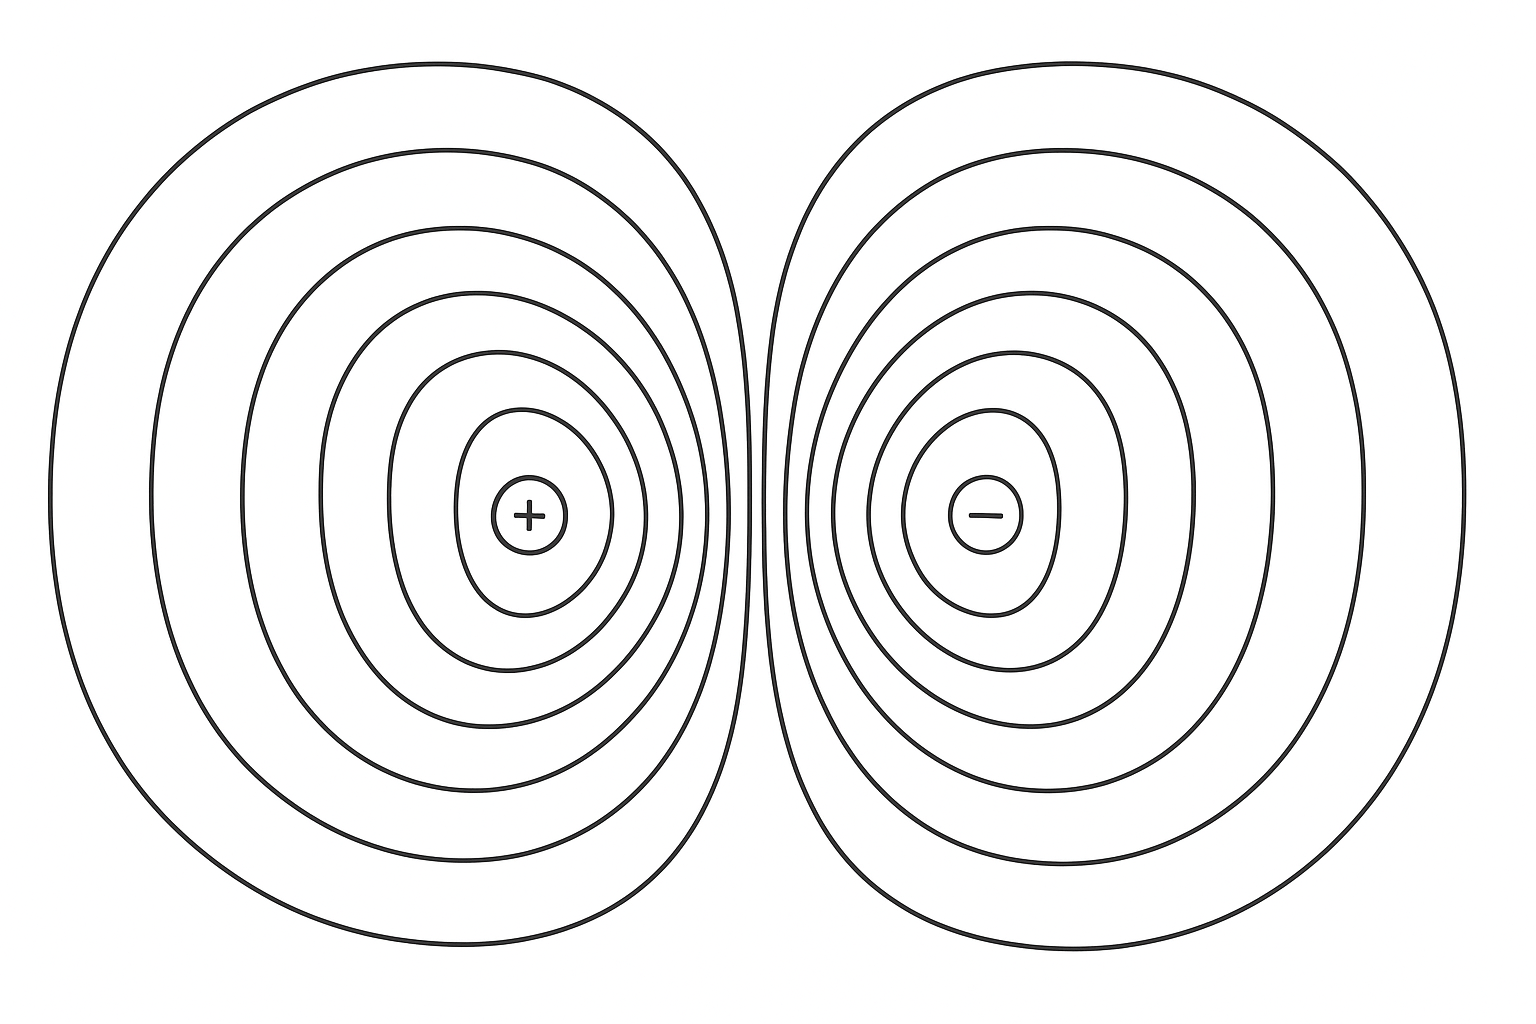
\includegraphics[width=0.75\linewidth]{rysunek2.png}
\caption{Przybliżony rozkład linii pola i linii ekwipotencjalnych dla dipola elektrycznego.}
\end{figure}

\subsection*{Przewodniki w polu elektrostatycznym}
W stanie równowagi elektrostatycznej wewnątrz przewodnika pole elektryczne jest równe zeru, ponieważ ładunki swobodne przemieszczają się po powierzchni tak długo, aż potencjał wyrówna się w całym przewodniku. W rezultacie, \textbf{linie pola elektrostatycznego są prostopadłe do powierzchni metalu} i kończą się na niej.
Rozkład ładunku elektrycznego występuje wyłącznie na powierzchni przewodnika, szczególnie w miejscach o dużej krzywiźnie (np. ostrzach), gdzie zagęszczenie linii pola jest największe.

\subsection*{Pole w kondensatorze płaskim}
Kondensator płaski tworzą dwie równoległe elektrody oddalone o odległość $d$. Między nimi powstaje w przybliżeniu \textbf{jednorodne pole elektryczne}, którego natężenie opisuje wzór:
\begin{equation}
E = \frac{U}{d}.
\end{equation}
Potencjał rośnie liniowo od elektrody uziemionej do dodatniej:
\begin{equation}
V(x) = \frac{U}{d}x.
\end{equation}
Poza przestrzenią między okładkami pole staje się niejednorodne i rozproszone.

\begin{figure}[h!]
\centering
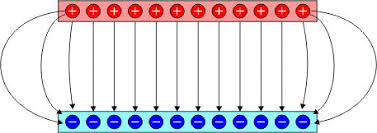
\includegraphics[width=0.7\linewidth]{rysunek3.jpeg}
\caption{Rozkład pola elektrycznego wewnątrz kondensatora płaskiego.}
\end{figure}

\subsection*{Czynniki wpływające na dokładność modelowania pola}
Dokładność modelowania pola elektrostatycznego zależy od kilku czynników:
\begin{itemize}
    \item jednorodności ośrodka przewodzącego (np. roztworu elektrolitu),
    \item dokładności wyznaczania potencjałów i stabilności napięcia zasilania,
    \item rozdzielczości siatki pomiarowej – im gęstsza, tym dokładniejszy wynik,
    \item precyzji wykonania i rozmieszczenia elektrod,
    \item wpływu brzegów i błędów pomiarowych woltomierza.
\end{itemize}

\section{Wzory}

\section{Aparatura pomiarowa}

\section{Wnioski}

\end{document}
